\section{The Basics of Nuclear Fusion and Tritium Breeding}\label{sec:fusion-basics}

\begin{figure}
	\centering
	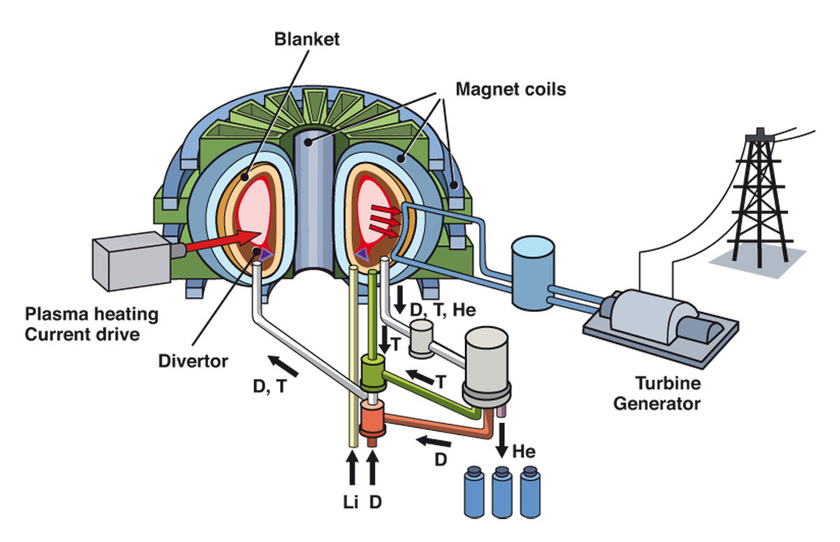
\includegraphics[width=0.85\textwidth]{chapters/figures/power-plant-schematic} 
	\caption{Schematic of a tokamak power plant showing the role of the blanket in both energy production and tritium breeding. (reproduced from the Max-Planck-Institut für Plasmaphysik)}
	\label{fig:power-plant-schematic}
\end{figure}

In Fig.~\ref{fig:power-plant-schematic}, we see the blanket surrounding the toroidally-shaped plasma and how the tritium generated in the blanket is recycled on-site to be fed back into the burning plasma. Also apparent in the sketch is the role of the breeding blanket as power generator. 


The most favorable fusion reaction for first generation tokamak-style fusion reactors involves the two hydrogen isotopes of deuterium and tritium. The deuterium-tritium (DT) reaction has a high reaction probability at the lowest ion temperature and a high energy yield. Alternative fusion reactions of two deuterium atoms or a deuterium atom with helium-3 are advantageous in other regards, such as no radioactive byproducts or fuel availability, but their relatively-higher ion temperature preclude them from current consideration.\cite{abdou} The DT reaction proceeds as
\begin{align}
	\mathrm{D} + \mathrm{T}&\xrightarrow{}\ ^4\mathrm{He}+\mathrm{n}+17.58\ \text{MeV} \label{eq:dt-reaction}
\end{align}

Of the two isotopes fused, deuterium ($D$, or $^2$H) is a stable isotope and is naturally occuring in an average abundance of 0.015 mole percent in water on Earth. To demonstrate just how plentiful deuterium is as a fuel source, there is approximately 100 million billion kilograms of deuterium in the Earth's oceans. If all energy on Earth were produced from DT fusion power plants, there would be enough deuterium to outlast the lifetime of our sun. We will not run out of deuterium.  

Tritium ($T$, or $^3$H), however, is radioactive with a half-life of only about 12.32 years; any naturally occurring tritium decays at such a rapid pace it will never accumulate to an appreciable amount on Earth. If tritium is to be used as a fuel in a fusion power plant, it must be generated artificially -- thus the need for the so-called tritium breeding blankets. In-situ generation of tritium in a fusion reactor is possible with the assistance of lithium. Natural lithium will interact with neutrons as
\begin{subequations}\label{eq:lithium-t}
\begin{align}
	\mathrm{n} + \ ^7\mathrm{Li} &\xrightarrow \ \mathrm{n}+\alpha + \mathrm{T} -2.47\ \text{MeV}\label{eq:li7-t}\\
	\mathrm{n} + \ ^6\mathrm{Li} &\xrightarrow \  \alpha + \mathrm{T} +4.78\ \text{MeV} \label{eq:li6-t}
\end{align}
\end{subequations}
where we have used the common short-hand of $\alpha$ in place of the helium nucleus. The cross-sections of the lithium reactions are given in Fig.~\ref{fig:li-xsects}. Note the exothermic lithium-6 reaction (a neutron of any energy will incite the transmutation) and the threshold energy required of the incident neutron in the endothermic lithium-7 reaction.

\begin{figure}
	\centering
	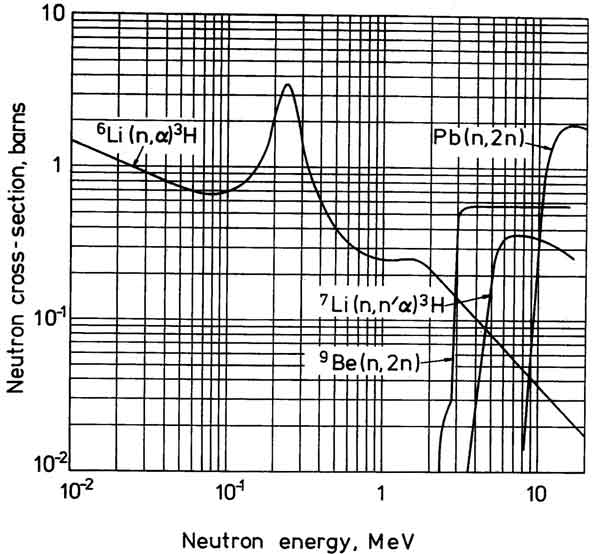
\includegraphics[width=0.75\textwidth]{chapters/figures/breeding_xsecs} 
	\caption{Cross-sections of various blanket materials. Note the threshold for the $^7$Li and neutron multiplying reactions.}
	\label{fig:li-xsects}
\end{figure}

Lithium, like deuterium, is quite abundant on Earth. To make the point clear, Francis Chen notes that there is enough lithium available on land to generate tritium for 30 million years of DT reactions providing all of humanity's electricity.\cite{Chen2011}. At the moment there are two main avenues of research for tritium breeder designs: liquid or solid lithium. While much research has been -- and continues to be -- performed on the liquid breeder design (for examples, see Refs.~[cite many liquid breeder papers]), the work of this dissertation focuses solely on the ceramic pebble beds populating solid breeder designs. Sketched in Fig.~\ref{fig:reactor-components} is the location of the breeding blanket and its relative location with other main components of a fusion reactor. 


\begin{figure}
	\centering
	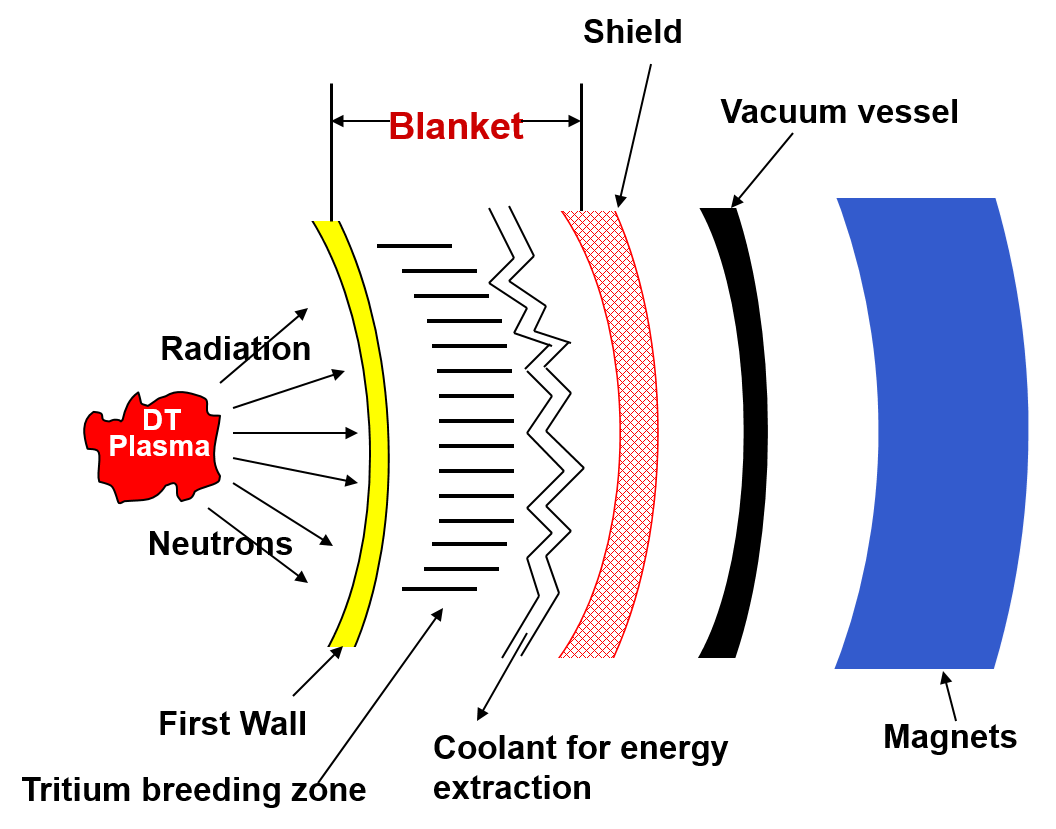
\includegraphics[width=0.85\textwidth]{chapters/figures/reactor_components.png} 
	\caption{Among the reactor components, the blanket and first wall are responsible for heat production and tritium generation.}
	\label{fig:reactor-components}
\end{figure}

